% ******************************* Thesis Appendix B ********************************

\chapter{Desaf\'ios t\'ecnicos encontrados}

% **************************** Define Graphics Path **************************
\ifpdf
    \graphicspath{{Appendix2/Figs/Raster/}{Appendix2/Figs/PDF/}{Appendix2/Figs/}}
\else
    \graphicspath{{Appendix2/Figs/Vector/}{Appendix2/Figs/}}
\fi

Durante la ejecuci\'on del proyecto, nos enfrentamos a desaf\'ios y en particular de carácter t\'ecnico. Dentro de estos desaf\'ios podemos encontrar algunos que se destacan por su complejidad y dificultad para resolverlos y otros que se destacan por su severidad como riesgo tecnol\'ogico dentro del proyecto. Por ello consideramos apropiado incluir un ap\'endice en donde se hace menci\'on a los mismos y a sus respectivas soluciones.

\section{Problemas con SFPs y Patchcoords}

Los transceivers SFP+ son una componente de hardware utilizada en cada puerto f\'isico de la tarjeta NetFPGA en la construcci\'on del dispositivo RAU-Switch. Básicamente se encargan de implementar el mecanismo de acceso a la capa f\'isica, en este caso fibra \'optica.

Pueden encontrarse transceivers compatibles con patch cords de fibra \'optica monomodo, multimodo y compatibles con ambos tipos.\\

En el desarrollo de este proyecto se trabaj\'o con transceivers SFP+ compatibles con ambos tipos de patch cords, aunque para la construcci\'on de la red prototipo por razones econ\'omicas se utilizaron transceivers SFP+ compatibles solamente con patch cords de fibra multimodo.


%Originalmente se trabaja con dos transceivers SFP+ compatibles con fibra monomodo y multimodo y patchords de f\'ibra \'optica monomodo, con los cuales se aprecia un correcto funcionamiento del hardware. 

%Posteriormente se incorporaron m\'as unidades de SFP+ con el objetivo de constru\'ir el laboratorio de pruebas descrito en el cap\'itulo \ref{chapter6}. En este caso se detectan problemas para establecer conexiones exitosas con cualquier nodo donde se utilice alguno de los SFP+ nuevos.\\

%La primera reacci\'on es de preocupación, ante la posibilidad de que la partida de SFP+ comprada estuviera fallada. Por ello se menciona el inconveniente en el grupo de trabajo generado GT-SDNUy, donde amablemente los integrantes del Centro de Desarrollo y Capacitacion de ANTEL comprueban el funcionamiento del hardware utilizando sus propios equipos.

%Tras comprobar que el hardware no se encuentra dañado, advirtiendo la posibilidad de que los SFP no sean compatibles con patch cords de fibra monomodo, el equipo de ANTEL nos facilita de patch cords multimodo, con los cuales posteriormente se constata el correcto funcionamiento de los SFP+.\\

%De esta forma, el laboratorio de pruebas queda implementado con SFPs compatibles solamente con fibra multimodo y patchcoords de fibra multimodo.

\section{Desprogramaci\'on del hardware NetFPGA}
\label{apendiceB2}

En el desarrollo de este proyecto se utilizan dos estrategias diferentes para programar el hardware NetFPGA. La primera estrategia, detallada en la guía de ejecución del Test de Producción\citep{ProdTestManual}, permite de forma sencilla programar el hardware utilizando la herramienta Impact de la suite Xilinx ISE SDK. Sin embargo este procedimiento no persiste la programaci\'on del hardware, por lo que al producirse un corte de corriente en el circuito (apagado de la PC por ejemplo) el mismo pierde la programaci\'on.

Este efecto puede comprobarse fácilmente utilizando la herramienta Impact para leer el valor de diferentes registros del hardware, los cuales indican el estado del mismo.\\

%Para la programación del hardware NetFPGA, se utiliza inicialmente el procedimiento indicado en el manual de ejecuci\'on del Test de Producci\'on ~\citep{ProdTestManual}. Tras experimentarse un tiempo con este procedimiento se constata que esta técnica de programación no es persistente. Esto significa que tras apagar y encender el equipo (ciclo completo de encendido) el mismo pierde la programación. 

%Utilizando la herramienta Impact, observando el comportamiento de LEDs en la placa y corroborando con el el manual de la misma, se constata que el contenido del chip CPLD se mantiene, pero el contenido del chip FPGA que si es eliminado.\\

La segunda estrategia es la programación PCIe denominada en este trabajo como programación persistente, la cual utiliza la herramienta \textbf{pcieprog} de la plataforma NetFPGA para almacenar la programaci\'on del hardware en una de las unidades de memoria Flash del equipo. Concretamente este procedimiento implica programar el hardware con un proyecto compatible con la programaci\'on PCIe (es necesario que el proyecto implemente un m\'odulo para la configuraci\'on del chip FPGA desde una de las memorias Flash) utilizando la herramienta Impact. Luego se almacena en una de las unidades de memoria Flash un archivo binario con la implementaci\'on del proyecto con el cual se quiere programar el hardware. Luego al momento del encendido del equipo, el chip FPGA es programado desde el contenido almacenado en una de las memorias Flash.

De esta forma la programaci\'on del equipo se almacena de forma persistente, perdurando incluso cuando el equipo es apagado.\\ 

%Con esta información se consulta la documentación de la plataforma y se buscan experiencias similares  de otros usuarios. No se encuentran problemas o experiencias similares pero se encuentra dentro de los proyectos de la plataforma un desarrollo de nombre Reference Flash, cuya funcionalidad es habilitar la programación persistente del hardware.

%Este proyecto utiliza las dos unidades de memoria flash disponibles, para almacenar la programaci\'on del equipo. Mientras que en la Flash A se almacena un bitstream de configuración para el equipo 
% (bootstrap bitstream), la  Flash B queda disponible para almacenar un bitstream a elección del programador. 

%La configuración del equipo es siempre manejada por el chip CPLD, el cual en el tiempo de encendido programa el chip FPGA con el contenido de la Flash A. Luego el equipo puede ser reprogramado desde la Flash B a través de la interfaz PCIe.

%Basándose en este proyecto, se prueba como solución al problema de la desprogramaci\'on del equipo dicha alternativa, utilizando como bitstream para la Flash B, el proyecto ReferenceNIC.\\

%Esta estrategia funciona  exitosamente en relación a la desprogramaci\'on del hardware, puesto que tal como su documentación lo indica se programa a partir del contenido de la Flash A; y luego utilizando la interfaz PCIe es existosamente reprogramada desde la Flash B. No obstante el comportamiento final del hardware no es el correspondiente al esperado por el proyecto ReerenceNIC. En particular tras reprogramar el equipo desde la Flash B no se puede insertar el driver para el ReferenceNIC en el kernel del sistema operativo (Linux).\\

%Tras utilizar el foro oficial de la plataforma, sin obtener respuestas se accede finalmente a una lista de correos en la que tambi\'en participan usuarios y desarrolladores de la plataforma. Aquí se explica el problema de la desprogrmaci\'on del hardware, y las alternativas exploradas. 

%Afortunadamente se obtiene respuesta del equipo de desarrolladores de NetFPGA, el cual nos indica que este comportamiento se debe a una incorrecta programaci\'on del hardware. Si bien se entiende correctamente la funcionalidad del proyecto ReferenceFlash, el proyecto ReferenceNIC precisa de módulos adicionales en el diseño de la CPLD que el ReferenceFlash no tiene. 

%Sin embargo, el proyecto ReferenceNIC ya tiene incorporado el modulo de persistencia que se presenta en ReferenceFlash. Por lo tanto, para lograr una programaci\'on persistente ademas de programar el equipo con el ReferenceNIC, se debe utilizar la herramienta \textbf{pcieprog} (dentro del mismo proyecto) para cargar en la memoria Flash A, un archivo bitstream con el contenido del mismo proyecto. De esta forma al producirse el encendido del equipo, este se programa con el contenido de la memoria Flash A.\\ 

%Esta es estrategia funciona correctamente, y es lo que en este trabajo se di\'o a conocer como programación persistente.

\section{Falta de licencias para suite de Xilinx ISE SDK}
\label{apendiceB3}
La suite de desarrollo Xilinx ISE SDK se compone por un conjunto extenso de herramientas para la progrmaci\'on y desarrollo de software utilizando los productos de este fabricante; entre los cuales se encuentra el chip Virtex 5 utilizado en el hardware NetFPGA.

Estas herramientas de software son licenciadas lo que significa que para su uso es necesario contar con una licencia de software apropiada.

Cada herramienta particular de la suite Xilinx tiene una licencia particular y se agrupan en diferentes paquetes de licencias. De esta forma dependiendo del uso que se vaya a hacer de esta plataforma, el o los paquetes de licencias que se deben adquirir. Adem\'as cada licencia se corresponde con una herramienta para una familia de chips en particular. Por ejemplo para trabajar con las tarjetas NetFPGA-10G se necesitan licencias para el chip Virtex5 TX240T.\\

Xilinx ofrece un paquete de licencias gratuitas para trabajar con un conjunto reducido de herramientas (entre ellas se incluye el programa Impact) y un paquete de licencias completo de prueba por un tiempo de 30 d\'ias compatible con los \'ultimos modelos de chips (Virtex6 y Virtex7). Como dentro de estos paquetes no se incluyen las licencias necesarias para la programaci\'on PCIe (programaci\'on persistente) una alternativa es adquirir un paquete de licencias con un valor aproximado de USD500 por PC (costo en dolares americanos al mes de Setiembre del año 2014).\\

%Si bien Xilinx provee de un paquete de licencias gratuito para un conjunto de herramientas mínimas dentro de la suite (entre estas se encuentra la herramienta Impact), en el desarrollo de este proyecto y en especial en el proceso de programaci\'on persistente del hardware se necesitan licencias para herramientas que no están incluidas en este paquete.

%A su vez, Xilinx provee de un paquete de licencias de prueba de 30 días en el cual se incluyen las herramientas necesarias para el proceso de programaci\'on persistente. No obstante en la familia de chips para las cuales este paquete de licencias provee de compatibilidad no se incluye la arquitectura del chip del hardware NetFPGA (mientras que la familia del hardware NetFPGA es Virtex5 TX240T, este paquete soporta familias de la arquitectura Virtex7).\\

%El conjunto de licencias necesarias para la ejecuci\'on de este proyecto se incluye en un paquete de licencias con un costo bastante elevado (al mes de Setiembre del año 2014 rondaba los USD500 aproximadamente por PC) y no hay un paquete de licencias gratuitas o de prueba que posibiliten la configuraci\'on del hardware NetFPGA de la manera pretendida en este proyecto.\\

En este proyecto, por razones econ\'omicas primero se solicit\'o mediante el programa de soporte a Universidades de Xilinx el paquete de licencias necesario, a la vez que se inici\'o un contacto con el Instituto de Ingeniería Eléctrica de la Facultad de Ingeniería (IIE) solicitando orientación en relación a este problema. 

Finalmente se recibi\'o a través de dicho programa de apoyo a universidades una interesante donación de licencias, posibilitando una real explotación del hardware y la plataforma en su conjunto, aunque esta espera represent\'o un contratiempo en el cronograma inicial del proyecto. 

%Tras este contacto se toma conocimiento que en el IIE no se trabaja actualmente con esta plataforma aunque en alg\'un momento si lo hicieron y gracias a ello se obtiene de parte de este instituto
%el asesoramiento y apoyo necesario para la resolución de este obstáculo. 

%Por otro lado, a través del programa de apoyo a universidades de Xilinx se obtiene una interesante donación de licencias, posibilitando a una real explotación del hardware y de la plataforma a futuro. Sin embargo, vale la pena destacar que esta donaci\'on se recibe bastante tiempo después de enviada la solicitud en dicho programa, y que estas licencias fueron un insumo necesario para continuar con la ejecuci\'on de este proyecto.  

\section{Falta de driver para cable JTAG Xilinx}
Para la programación del hardware NetFPGA se utiliza un cable programador especial con una interfaz de conexi\'on JTAG.  Este cable presenta el inconveniente de que sus fabricantes no desarrollaron drivers para la distribución de Linux con la que se trabaja en este proyecto, existiendo drivers oficiales para entornos Windows y una versi\'on no oficial para la distribución Fedora.\\

Si bien inicialmente esto oblig\'o a programar el hardware en un ambiente Windows para realizar las pruebas de verificaci\'on del mismo (Producction Test y RLDRAM Test) finalmente se consigue un driver no oficial\cite{JtagD} tambi\'en compatible con Ubuntu 12.04, habilitando de esta forma a programar el hardware en la misma PC.

%Por un lado, para utilizar este cable es necesario instalar un driver especifico para el mismo. Para la marca de cable JTAG utilizado en este proyecto (Xilinx) el driver oficial provisto por el fabricante tiene soporte solamente para sistemas Windows.

%A pesar de que existe una implementaci\'on de este driver para sistemas basados en GNU/Linux (la cual no guarda relación con el fabricante), se prueba en este proyecto que funciona solamente en Fedora.\\

%Finalmente luego de un esfuerzo mayor buscando una implementaci\'on de driver compatible con Ubuntu 12.04 se encuentra la implementaci\'on \cite{JtagD}, la cual tras bajar el codigo fuente y compilarlo apropiadamente, se puede utilizar el cable de programaci\'on JTAG exitosamente.

\section{Problemas t\'ecnicos con Open vSwitch}
\label{apendiceB5}

Open vSwitch es uno de los pilares fundamentales de RAU-Switch puesto que es el encargado de implementar el plano de datos de OpenFlow. Durante el desarrollo de este proyecto, en el tiempo empleado a la experimentaci\'on con esta herramienta, se genera conocimiento en relaci\'on a aspectos importantes sobre la herramienta; los cuales no son triviales y vale la pena mencionar en este apartado. A continuaci\'on se enumeran los siguientes:\\ 

\begin{enumerate}
\item Parte de las funcionalidades de Open vSwitch, est\'an implementadas en modo kernel y otra parte en modo usuario. Estas \'ultimas presentan un nivel de performance muy pobre en comparaci\'on a las primeras; y en particular las funcionalidades de MPLS se encuentran solamente disponibles en modo usuario.

\item De acuerdo a la p\'agina de preguntas frecuentes, la \'ultima versi\'on de Open vSwitch al momento de realizarse este proyecto, garantiza soporte a las operaciones de MATCH, PUSH y POP de hasta tres etiquetas MPLS apiladas, as\'i como su posterior procesamiento acorde al pipe de OpenFlow. Todas estas funcionalidades adem\'as se implementan en modo usuario.\\

Por otro lado, de acuerdo  a las notas de liberaci\'on de la versi\'on 2.3.1, solamente se garantiza el soporte a las funciones de MATCH, PUSH y POP de MPLS para un \'unico nivel de etiquetas; esto es una sola etiqueta MPLS. Luego se garantiza adem\'as el posterior procesamiento acorde al pipe OpenFlow.\\

Esta informaci\'on no s\'olo es contradictoria, sino que adem\'as no se condice con la realidad. Experimentalmente se prueba que si bien la versi\'on 2.3.1 implementa correctamente las operaciones de MATCH y PUSH de una \'unica etiqueta MPLS, la operaci\'on POP no se encuentra implementada para esta versi\'on, rompiendo adem\'as el pipe de procesamiento OpenFlow. 

Afortunadamente \'este comportamiento hab\'ia sido detectado y reportado por otros usuarios de Open vSwitch como un BUG, resolviéndose posteriormente en la versi\'on de desarrollo~\citep{OVSSourceCode}.

\item Trabajando con la versi\'on de desarrollo en el repositorio de c\'odigo fuente de Open vSwitch~\citep{OVSSourceCode} (rama master en el repositorio Git), se comprueba experimentalmente el soporte para las operaciones de Match, Push y Pop de hasta 3 etiquetas, as\'i como el posterior procesamiento del paquete seg\'un el pipe de  OpenFlow.

\item Puertos OpenFlow con direcciones IP:
%Una condici\'on necesaria en la arquitectura del prototipo es la capacidad de asignar direcciones IP a cada interaz del router opensource.
 
Para lograr que cada interfaz f\'isica de la tarjeta NetFPGA se comporte tanto como un puerto OpenFlow, como una interfaz IP, es necesario:

\begin{enumerate}
\item Crear un bridge con Open vSwitch y agregar cada interaz f\'isica como un puerto OpenFlow al mismo.
\item Asignar una dirección IP a la propia intefaz f\'isica (por ejemplo utilizando el comando ifconfig).
\end{enumerate}

%Debido al comportamiento de un bridge en Linux, esta estrategia que parece natural e inmediata, no se comporta en la pr\'actica como se necesita en este proyecto. El comportamiento deseado de una interfaz h\'ibrida IP/OpenFlow en el prototipo ser\'ia el que se indica en la figura~\ref{fig:OVSInterfaces}.

El comportamiento deseado por una interfaz h\'ibrida IP/OpenFlow en el prototipo ser\'ia el que se muestra en la figura ~\ref{fig:OVSInterfaces} (mitad izquierda).

El paquete ingresa al router atrav\'es de la interfaz f\'isica \textbf{nf0} y de ah\'i en m\'as el procesamiento del mismo es delegado al m\'odulo de Open vSwitch en el kernel de Linux. Aqu\'i el paquete es procesado y tratado en consecuencia a lo que indica la tabla de flujos en Open vSwitch. En el prototipo, para este paquete existen dos alternativas: (1) se procesa el contenido del mismo y se reenv\'ia por otra interfaz acorde a la regla correspondiente, (2) es contemplado por una regla con la acci\'on \textit{NORMAL} y por tanto es procesado como lo har\'ia un switch legado (en este caso como lo procesar\'ia el kernel de linux).\\

\begin{figure}[h!] 
\centering    
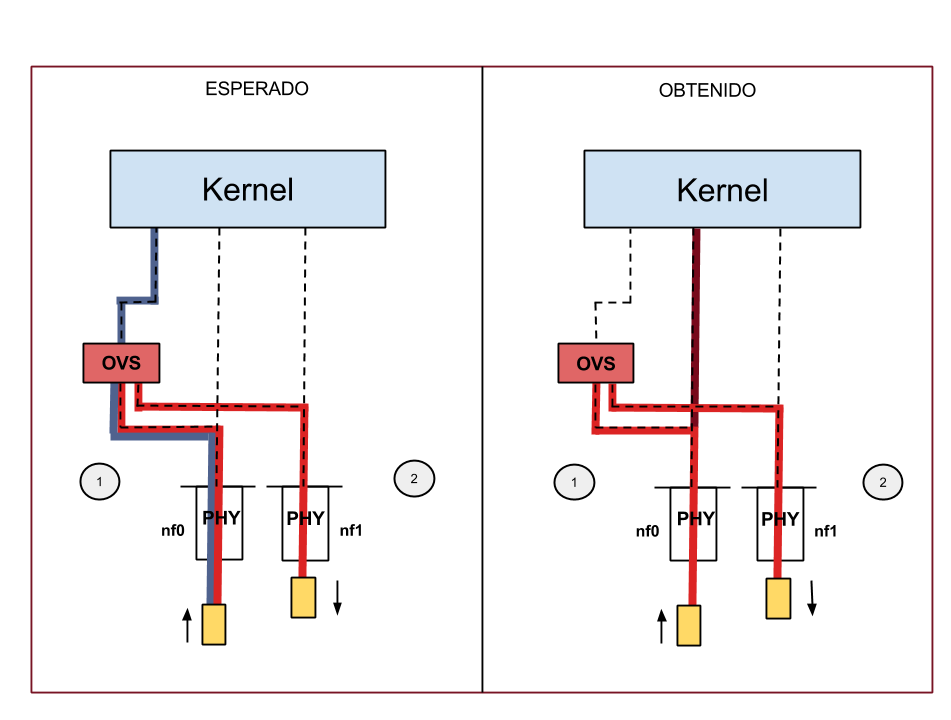
\includegraphics[width=0.65\textwidth]{ovs_figure3}
\caption[Funcionamiento de puertos Open vSwitch]{Funcionamiento de puertos Open vSwitch}
\label{fig:OVSInterfaces}
\end{figure}

No obstante, el procesamiento del paquete al ingresar por la interfaz f\'isica \textbf{nf0} difiere del comportamiento deseado (ver mitad derecha de la imagen). El paquete es procesado por Open vSwitch como se describi\'o anteriormente, pero tambi\'en es enviado para su procesamiento en el kernel de Linux.

Esto implica que el switch se comporte como una mezcla de un switch OpenFlow  con una PC Linux normal, ocasionando un tratamiento de paquetes en el prototipo diferente al especificado por las reglas OpenFlow calculadas.\\

Para solucionar este problema se utilizan interfaces virtuales de la siguiente forma:

\begin{enumerate}
\item Se crea una interfaz virtual por cada interfaz física y se conecta a través de dichas interfaces,  openvswitch con el kernel.

\item La dirección IP que antes se asignaba a cada interfaz física ahora se le asigna a su correspondiente interfaz virtual.

\item Se deja la interfaz física sin dirección IP y de esta forma se asegura que ningún paquete que arribe a dicha interfaz será procesado por el kernel, ya que nunca coincidirá la dirección IP que contenga un paquete con la dirección de la interfaz.

\item Se crean entradas de prioridad mínima en la tabla de flujos de openvswitch que indiquen que todo lo que entre por la interfaz física se envíe a través su correspondiente interfaz virtual y viceversa.

\item De esta forma si no hay un flujo de mayor prioridad para procesar los paquetes que entran por determinada interfaz física, estos serán enviados al kernel mediante la interfaz virtual, procesados por este para luego ser enviado por la interfaz virtual a la física y seguir su camino.

\item Estos pasos aseguran que todo el tráfico sea procesado por las tablas de Open vSwitch, y serán procesados por el kernel solo en caso de ser necesario.
\end{enumerate}

\begin{figure}[h!] 
\centering    
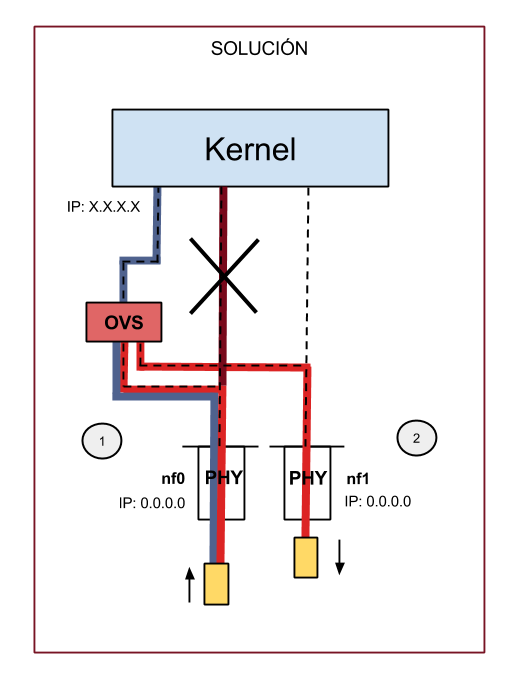
\includegraphics[width=0.35\textwidth]{ovs_figure4}
\caption[Puertos Open vSwitch - Soluci\'on propuesta]{Puertos Open vSwitch - Soluci\'on propuesta}
\label{fig:OVSInterfaces2}
\end{figure}

\end{enumerate}

\newpage
\section{MPLS Linux y Quagga LDP}
\label{apendiceB6}

MPLS Linux es un proyecto orientado a dotar de funcionalidades de MPLS al Kernel de Linux, mediante un parche con el cual se extiende al mismo y el cual tras recompilarse queda pronto para brindar soporte nativo al protocolo MPLS. %Adicionalmente es necesario instalar herramientas para por ejemplo acceder a las tablas de MPLS (en particular existe una extension de la herramienta iproute denominada iproute2 para esto).\\

Existen principalmente dos versiones: el proyecto original\cite{MplsLinux1} encabezado por James R. Leu el cual data de hace m\'as de 15 a\~nos y no cuenta con contribuciones importantes desde hace aproximadamente 9 y otro proyecto\cite{MplsLinux2} encabezado por Igor Maravick (quien trabaj\'o en el proyecto anterior) que data del a\~no 2010 y surge como una actualizaci\'on del proyecto original.\\

El primer proyecto fue pensado como un parche para el kernel de Linux versi\'on 2.6.3.16 (tener en cuenta que la versi\'on actual es la 4.1.1). Adicionalmente se desarroll\'o una extensión de la suite Quagga\cite{QuaggaLDP1} que implementa el algoritmo LDP para la construcci\'on de redes IP/MPLS.

Por otro lado, el proyecto de Igor Maravick es un kernel de Linux versi\'on 3.9.0-rc3 con las modificaciones necesarias para soportar el protocolo MPLS ya incorporadas. Adicionalmente existe una nueva extension de la suite Quagga que implementa el protocolo LDP \cite{QuaggaLDP2} y es compatible con esta versi\'on de MPLS-Linux.\\

En el contexto de este proyecto se trabaj\'o con ambas versiones de MPLS-Linux y las respectivas versiones de Quagga-LDP. 

Para la versi\'on original de MPLS-Linux se prob\'o compilar el parche con diferentes versiones de kernel, entre ellas las versiones 2.6.32.16 y 2.6.32.65 no pudiendo as\'i configurar correctamente el ambiente de trabajo. En particular estas versiones son tan antiguas que gran parte de las herramientas utilizadas para la construcci\'on de RAU-Switch no son compatibles. Adicionalmente se prueba compilar el parche para la versi\'on de kernel 3.11.0-15 generic (versi\'on que trae Ubuntu 12.01) pero tampoco se obtienen buenos resultados.\\

En relaci\'on a la versi\'on de Igor Maravik se logr\'o configurarla correctamente, as\'i como la extensi\'on Quagga-LDP. No obstante al momento de ejecutar dichas herramientas se detectaron problemas en la interacci\'on entre las mismas; mediante los logs de la herramienta Quagga se detectaron errores al momento de insertar entradas en las tablas MPLS del kernel.

Finalmente por la falta de información en relación a estas componentes, ya que sobre el proyecto original existe muy poca documentaci\'on mientras que para el proyecto de Igor Maravik no existe la misma, se decidi\'o descartar esta alternativa para implementar el algoritmo LDP. 


%El proyecto, cuyo desarrollo fue encabezado por James R. Leu, data de hace m\'as de 15 a\~nos y no se han hecho contribuciones importantes desde hace aproximadamente 9. Adem\'as de que la documentaci\'on existente es muy poca, las versiones de kernel de Linux para las cuales se pensó este parche rondan por la versi\'on 2.6.3.16, cuando la \'ultima versi\'on de kernel es la 4.1.1.\\

%Durante la ejecuci\'on de este proyecto, se prueba instalar este parche en dos kernel de Linux contemporáneos (versi\'on 2.6.32.16 y 2.6.32.65) obteniendo resultados no satisfactorios. Concretamente estas versiones de kernel son tan antiguas que no soportaron algunas características del hardware utilizado para la contrucci\'on de RAU-Switch, adem\'as de que tampoco soportan completamente la herramienta Open vSwitch.

%Se prueba compilar este parche en la versi\'on de kernel con la que se estaba trabajando hasta el momento (3.11.0-15 generic) pero sin resultados satisfactorios.\\

%Cabe desatacar que para esta versi\'on de MPLS-Linux el mismo autor, James R. Leu desarroll\'o una extension de la suite Quagga para trabajar con MPLS-Linux y el protocolo LDP, lo cual se dio a llamar Quagga LDP\cite{QuaggaLDP1}.\\  

%Por otro lado, Igor Maravick; quien trabajara junto a James R. Leu en el desarrollo de MPLS-Linux, decide retomar este proyecto y actualizarlo a una versi\'on de kernel de linux m\'as actual. 

%Lo que comenzó en el a\~no 2010 como un proyecto para portar MPLS-Linux termino en el a\~no 2013, en prácticamente una reimplementaci\'on del proyecto original utilizando un kernel versionn 3.9.0-rc3. 

%Como gran diferencia del proyecto original adem\'as, no se incluye MPLS-Linux como un parche si no que viene integrado en la propia distribución.\\

%En el contexto del proyecto, tras varias semanas de esfuerzo se logra configurar, compilar e instalar \'este kernel con la configuraci\'on del kernel con la que se ven\'ia trabajando al momento, garantizando as\'i el correcto funcionamiento del resto de las herramientas de software y hardware instaladas, entre las cuales se encuentran principalmente el hardware NetFPGA. Conviene resaltar que la documentaci\'on existente sobre este proyecto es prácticamente nula, adem\'as de que al cambiar la implementaci\'on del proyecto, la documentaci\'on del proyecto original no sirve.\\

%Por otro lado, puesto que la implementaci\'on original de Quagga LDP realizada por James R. Leu no es compatible con esta versi\'ion de MPLS-Linux, es necesario encontrar una versi\'on que si lo sea. Afortunadamente, contemporáneo con el proyecto de Igor Maravic, se origina un proyecto\citep{QuaggaLDP2} para portar la versi\'on original de Quagga LDP a la implementaci\'on de MPLS-Linux m\'as reciente.\\

%En el contexto del proyecto se compila e instala esta implementaci\'on de Quagga y nuevamente tras largos esfuerzos (recordar que casi no existe documentación) se logra ejecutar correctamente. 

%No obstante al momento de integrar ambas herramientas surgieron problemas, concretamente en los logs del demonio zebra se detectaron errores al momento de insertar entradas en las tablas MPLS del kernel de Linux, y tras varias semanas de buscar informaci\'on en la web, analizar el error e inspeccionar el código fuente en busca de alguna pista, se descarta la alternativa de utilizar MPLS-Linux y Quagga LDP en el prototipo. 
